\documentclass{article}
\usepackage[utf8]{inputenc}
\usepackage[T1]{fontenc}
\usepackage[english]{babel}
\usepackage{amsmath}
\usepackage{amssymb,amsfonts,textcomp}
\usepackage{array}
\usepackage{hhline}
\usepackage{hyperref}
\usepackage{graphicx}

\let\oldsection\section
\renewcommand\section{\clearpage\oldsection}

\newcommand{\pitem}[1]{
	\item{\textbf{#1}}
}

\graphicspath{ {./images/} }

\begin{document}
	\title{Croud \\ \vspace{2 mm} {\large A non-technical geographic crowdsourcing framework}}
	\author{Samuel Gaus}
	\date{1\textsuperscript{st} May 2015}
	\maketitle

	\tableofcontents

	\section{Summary}
	\label{sec:summary}
		Geographical data collection is a commonly-repeated task in scientific research, political campaigning, land administration and humanitarian projects.
		At the moment, there are a number of solutions for organisations wishing to go about data collection, from using existing frameworks to commissioning bespoke software.
		However, these are either extremely technical, overly generic (i.e. not specifically suited to collecting geographic point data) or expensive to implement.

		This document will show that in essence most organisations have very similar requirements for their data collection and as such it is possible to engineer a solution that is abstract enough to be used in many different fields.
		After analysing a number of potential benefactors, a framework was produced, set of APIs and mobile app that can be used by anyone requiring a crowdsourcing campaign to start collecting data in minutes.

		The framework that has been produced could be applied to collecting data on potholes just as easily as it could be used to help volunteers map out crisis-prone areas of the world.

	\section{Introduction}
	\label{sec:introduction}
		\subsection{Problem}
		Data collection is a very common task in computer science and software development. The requirement to gather information from disparate human sources (or crowdsourcing) can be found from everywhere research projects to humanitarian missions.

		\subsection{Current Situation}
		At the moment individuals or organisations looking to initiate a campaign of data collection either have to start their project from scratch or use one of the extremely abstract frameworks available.
		The framework with the widest reach is \emph{PyBOSSA}, a crowdsourcing platform inspired by \emph{BOSSA} and written in Python. \emph{BOSSA} is a front-end written in PHP to provide a web-based client for \emph{BOINC}, the software behind hundreds of data collection projects such as \emph{SETI@home}, \emph{World Community Grid} and \emph{Climate Prediction}\cite{_boinc_2015}.
		PyBOSSA is a rewrite of that with a focus on helping scientists and other researchers crowdsource human problem-solving skills.

		Alternatively, some organisations have produced their own bespoke software. In 2007, \emph{mySociety} made FixMyStreet - a platform for ``reporting common street problems such as potholes and broken street lights''\cite{_mysociety/fixmystreet_2015}.
		A user needs only to click on a map, fill in a survey and submit and the report is sent to the relevant council authority.
		This system was released open-source for any council to host and use, and theoretically for anyone to adapt to their own crowdsourcing needs.

		There are a number of issues present in using the existing solutions of \emph{PyBOSSA}, \emph{FixMyStreet} or bespoke software. Firstly, for all three there is a technical knowledge requirement. \emph{PyBOSSA} and \emph{FixMyStreet} both need server space, system administration to install and maintain and all the skills required for any necessary customisations.
		\emph{crowdcrafting} is a platform powered by the \emph{PyBOSSA} framework which is free to use and allows a user to set up a \emph{PyBOSSA} campaign without the aforementioned requirements.
		However, even in this case, there is significant technical knowledge required to set up a geographic data-collection campaign due in part to the level of abstraction that the project has achieved from the types of data it could be used to collect.
		A campaign creator must create a form in \emph{HTML} for the data collection, and the user does not get easy access to a map to just drop their pin. Requiring technical skill to operate the software means that in order to run a campaign one either needs a specific skill set or the financial resources necessary to pay a third party.

		There is no way to validate data input using this method.
		For example, you may have a field of data collection in your campaign that must be numerical.
		Although you can use the \texttt{number} input type in \emph{HTML}, this doesn't stop an old browser or malicious user sending non-numerical data in the response.

		The data submission in \emph{PyBOSSA} is very much a one-way street in terms of availability. This means that the data visibility is low for the user and high for the campaign owners. Many crowdsourcing solutions (for example FixMyStreet) have a much more balanced data visibility, where both users and owners can see the data that has been submitted so far.

		Finally, although existing systems could be used hypothetically with enough technical skill for most crowdsourcing campaigns, they would still take a lot of time to prepare. In some applications of crowdsourced data collection time taken to set up a campaign is an extremely important factor. For example, when Malaysian Airlines Flight 370 crashed in 2014, there was an immediate rush of humanitarian workers to find the location of the plane. Enormous stretches of sea were inspected remotely by ``citizen scientists'' within days due to the existence of \emph{Tomnod} - a crowdsourcing platform built around distributed human inspection of images (in this case satellite images)\cite{_missing_2014}. Because a crowdsourcing framework was already in place specifically for that sort of data analysis, they were able to be more responsive than the government organisations expending huge resource on similar endeavours.

		\subsection{Proposal}
		In the previous sections we have seen that there a number of projects that have been created to crowdsource data from users in the field. We have also seen from \emph{Tomnod} that pre-existing frameworks that are highly specialised are extremely important for easily setting up data collection campaigns quickly and cheaply. Would it be possible to create a framework targeted and tailored specifically for distributed data collection in the field?

		\subsection{Structure}
		This document will show that it is indeed possible to create an easy-to-use, quick and open crowdsourcing framework. It will show that when the data collection requirements are focussed on geographic data, efforts from anyone looking to crowdsource could be reduced dramatically.

		First the \hyperref[sec:background]{background} of crowdsourcing and ``citizen science'' will be discussed in more depth. The number of projects that could benefit from a common framework and determine the common functionalities will be assessed. These functionalities will be compared with the features of currently-available frameworks and will show, as a result that the framework that will be proposed would be an original work benefiting users and campaign-creators alike.

		Once the set of required features is clear, the document will go into more detail about the \hyperref[sec:architecture]{architecture} used to create such a framework. A more detailed explanation of what the framework actually is will be given and a comprehensive requirements analysis to which the project could be built will be supplied. The document will show how the different components fit together and how it works overall. The specific technologies that have been implemented will then be justified and elaborated upon.

		The document will then provide more information on the actual \hyperref[sec:implementation]{implementation} of the software complete with source code. It will go through the schemas used in the data storage and some key snippets from the source code. It will also provide information on some of the features that would be more challenging for any other party attempting to reproduce the framework.

		In order to show that the framework is appropriately constructed, it will be \hyperref[sec:evaluation]{evaluated} against two completely separate potential campaigns and shown that it is suited to the requirements of both. This section will contain a walkthrough of the creation of a campaign with screenshots, and then the same for submitting data to a campaign.

		In \hyperref[sec:conclusion]{conclusion}, some future improvements on the framework and associated applications will be explored and recommended and an analysis on what worked and why will be provided.

		The software produced to show this was named \emph{Croud}, a portmanteau of ``cloud'' and ``crowd''. It is hosted on \href{http://croud.io/}{\texttt{http://croud.io/}} - please feel free to visit and try it out for yourself.

	\section{Background}
	\label{sec:background}
		\subsection{Crowdsourcing}
		Crowdsourcing is a term coined in 2005 by editors of \emph{Wired Magazine} Jeff Howe and Mark Robinson\cite{safire_fat_2009} referring to the outsourcing of a task to the crowd. The rise of the internet and of mobile phones has made crowdsourcing an extremely efficient way of collecting data on a large scale. Due in part to its relevance to both business and academic research, it has been subject to a vast quantity of study of both its effectiveness\cite{brabham_effectiveness_2010} and the techniques of motivation that draw people to participating\cite{hossain_users_2012}. Much of this study is part of research focussing on \emph{computer-supported cooperative work}, a more general topic covering software that helps groups of people work together in ways that would not be possible or worthwhile without technology.

		When applied to gathering data for research, crowdsourcing is a form of citizen science\cite{_citizen_2015}. In this field, however, there is a more specific definition given to crowdsourcing. Muki Halay describes crowdsourcing as ``level 1'' of participation in citizen science, where a citizen merely acts a sensor. In higher levels, citizens contribute to data interpretation (``distributed intelligence''), problem definition (``participatory science'') and data analysis (``extreme citizen science'')\cite{haklay_citizen_2013}.

		\subsection{Existing projects}
		There are a growing number of projects that involve crowdsourcing geographic information. Although there are many to choose from, information will be provided for a few that roughly represent the disparate use cases.

		\paragraph{OpenStreetMap}
		\emph{OpenStreetMap} (\emph{OSM}) is a world-wide online collaborative effort to create detailed maps of the world under a free\cite{_open_2012} license started in 2004. Any user from around the world can submit geographic data using either the web-based application, or offline tools like \emph{Merkaartor}. Although used by individuals and organisations everywhere, it has also been crucial in ``crisis mapping''. Since the Haiti earthquake in 2010, volunteers have provided geographic data on areas experiencing crises to \emph{OSM} to help humanitarian workers\cite{_our_????}. This effort has since expanded into the Missing Maps project, within which the \emph{Humanitarian OSM Team} work with \emph{Medecins Sans Frontieres} and the \emph{American Red Cross} to pre-emptively map ``the most crisis-prone parts of the developing world''\cite{_missing_????}.

		\paragraph{FixMyStreet}
		\emph{FixMyStreet} is - a platform for ``reporting common street problems such as potholes and broken street lights''\cite{_mysociety/fixmystreet_2015} created by \emph{mySociety} in 2007. \emph{mySociety} is an ``e-democracy'' charity in the UK that have created and operate a number of tools to improve the user experience of national and local government. \emph{FixMyStreet} in particular is used to simplify the process of reporting potholes, broken street lamps etc. to their local authority. Users submit a description of the problem attached to a coordinate pair via the website or mobile applications for \emph{Android} and \emph{iOS}. It has been adopted by local authorities all over the world.

		\paragraph{Fill That Hole}
		\emph{Fill That Hole} is a cyclist-specific app for reporting potholes to the relevant Council in the UK. It differs from other reporting systems because the data submitted is public and freely usable by other systems via and API. For example, the journey planner \emph{Cyclestreets} takes the potholes reported on \emph{Fill That Hole} into account when planning routes. Reports are submitted via mobile applications for \emph{Android} and \emph{iOS}.

		\paragraph{Cyclestreets}
		Although basing most of its data on \emph{OSM}, the cyclist journey planner \emph{Cyclestreets} also hosts a ``Photomap'' where users are encourage to upload geolocated photographs of cycling infrastructure. This data is used to affect route planning and the provided images themselves are appended to route itineraries\cite{_cyclestreets_????}.

		\subsubsection{Common functionalities}
		\label{sec:common-functionalities}

		The projects listed above share a number of functionalities. They are isolated and listed here, although every project does not require every functionality.

		\begin{itemize}
			\item Interface to submit some validated payload of form data with an accompanying coordinate pair.
			\item User is free to submit data for any location without restriction (although data may be moderated afterwards).
			\item Users can submit as much data as they like - they can be power users or occasional users.
			\item Some means of displaying the submitted data on a map. This may be as a set of markers, icons or a heatmap.
			\item Ability to export the collected data in a machine-readable format.
			\item When data is submitted by anonymous or unknown users, it may require moderation either due to being false, because it needs editing or because the data is no longer relevant.
			\item A well documented API covering all of this functionality. Typically these tools exist as part of a chain of software; they need a good machine interface to be able to receive data in as many ways as possible, and to share their collected data as required.
		\end{itemize}

		\subsection{Available frameworks}

		The field of crowdsourcing is not without existing frameworks. The key offering currently available is \emph{PyBOSSA}, already introduced in section \ref{sec:introduction}.

		\subsubsection{PyBOSSA}

		\emph{PyBOSSA} is available without requiring server space through \emph{crowdcrafting}. The following will briefly cover the process for creating a geographic in-the-field data collection project using \emph{crowdcrafting}, and will show that the framework is not fully compatible with the field of crowdsourcing projects addressed in this study.

		\begin{enumerate}
			\item Create a user account on the website.
			\item Start a new `Project' (Figure \ref{fig:cc-create}).
			\item `Import' some `Tasks'.\\
			\emph{crowdcrafting} is designed to atomize tasks and distribute them between contributors. In order to achieve this, it requires a CSV (or Google Spreadsheet or similar) of `Tasks'. For example, in the geographic data example they provide for ``Urban Parks'', the tasks are questions like ``Find an urban park for this city'', along with a city name\cite{_urban_????}. To make the system cater for the kind of campaign discussed in this project, the file provided here would need to be consist of a singular question.
			\item Edit the `Task Presenter' to be both mobile-compatible and capable of using geolocation as well as pointing to where you are on a map (Figure \ref{fig:cc-present}).
			\item Publish the Project.
		\end{enumerate}

		\begin{figure}[hb]
			\centering
			\fbox{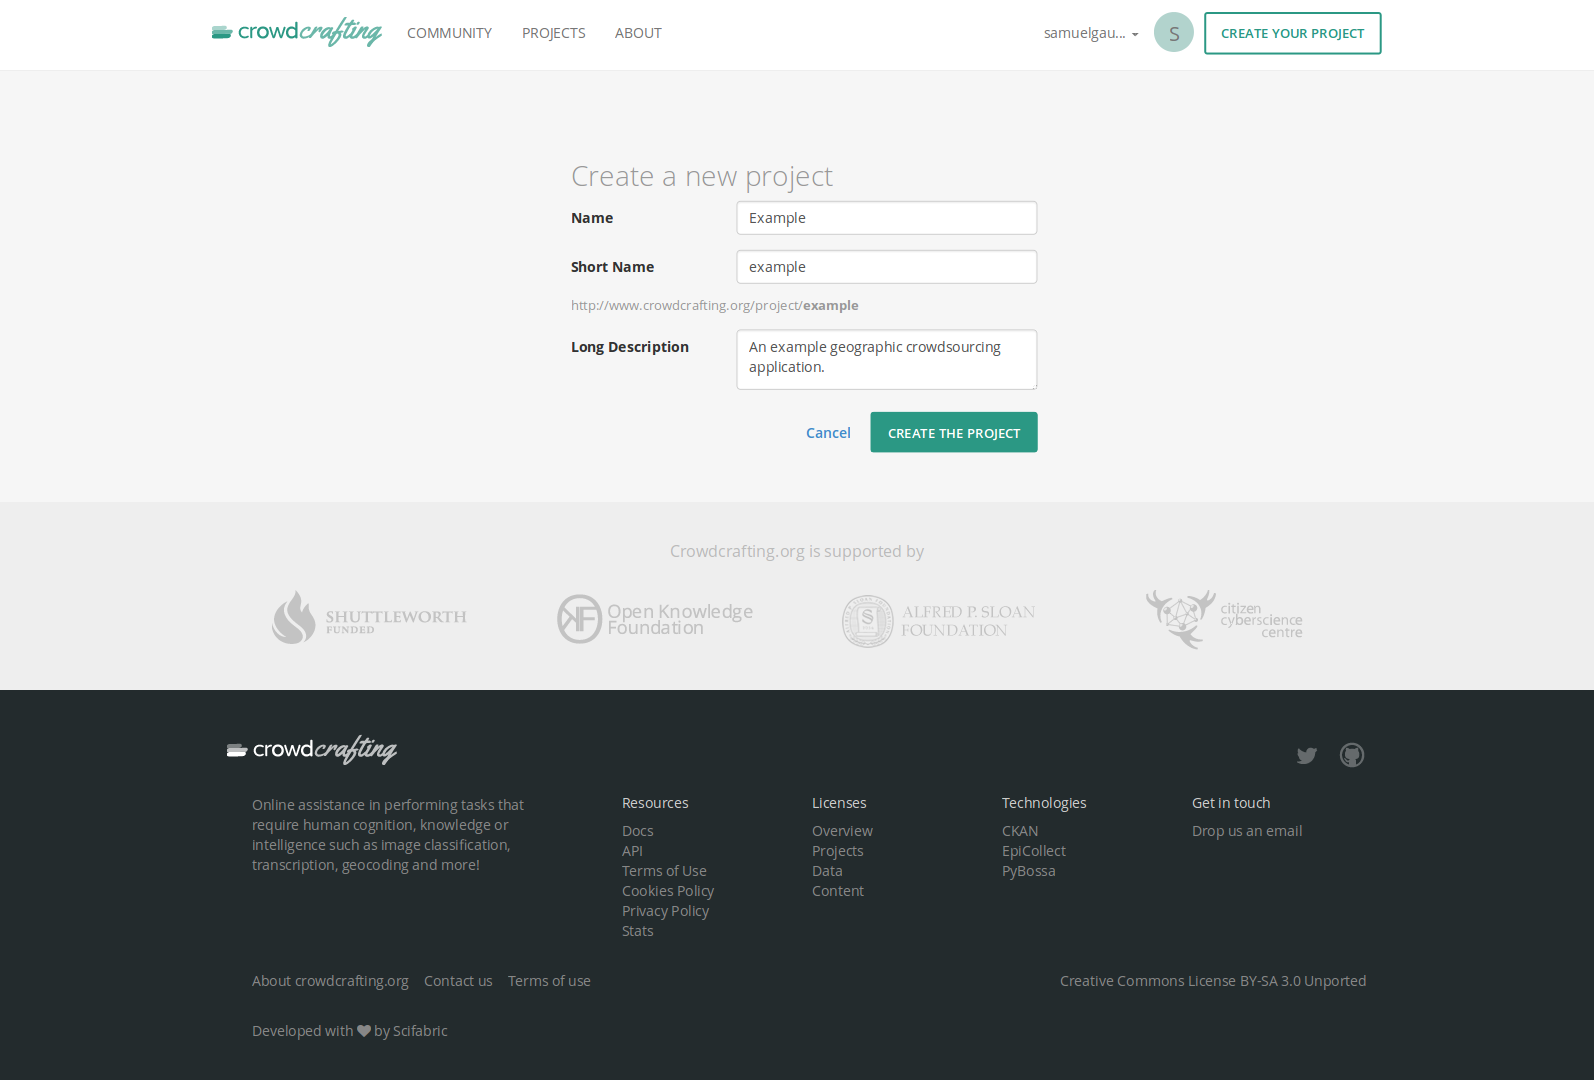
\includegraphics[width=4in]{cc-create}}
			\caption{Creating a project in \emph{crowdcrafting}}
			\label{fig:cc-create}
		\end{figure}

		\begin{figure}[hb]
			\centering
			\fbox{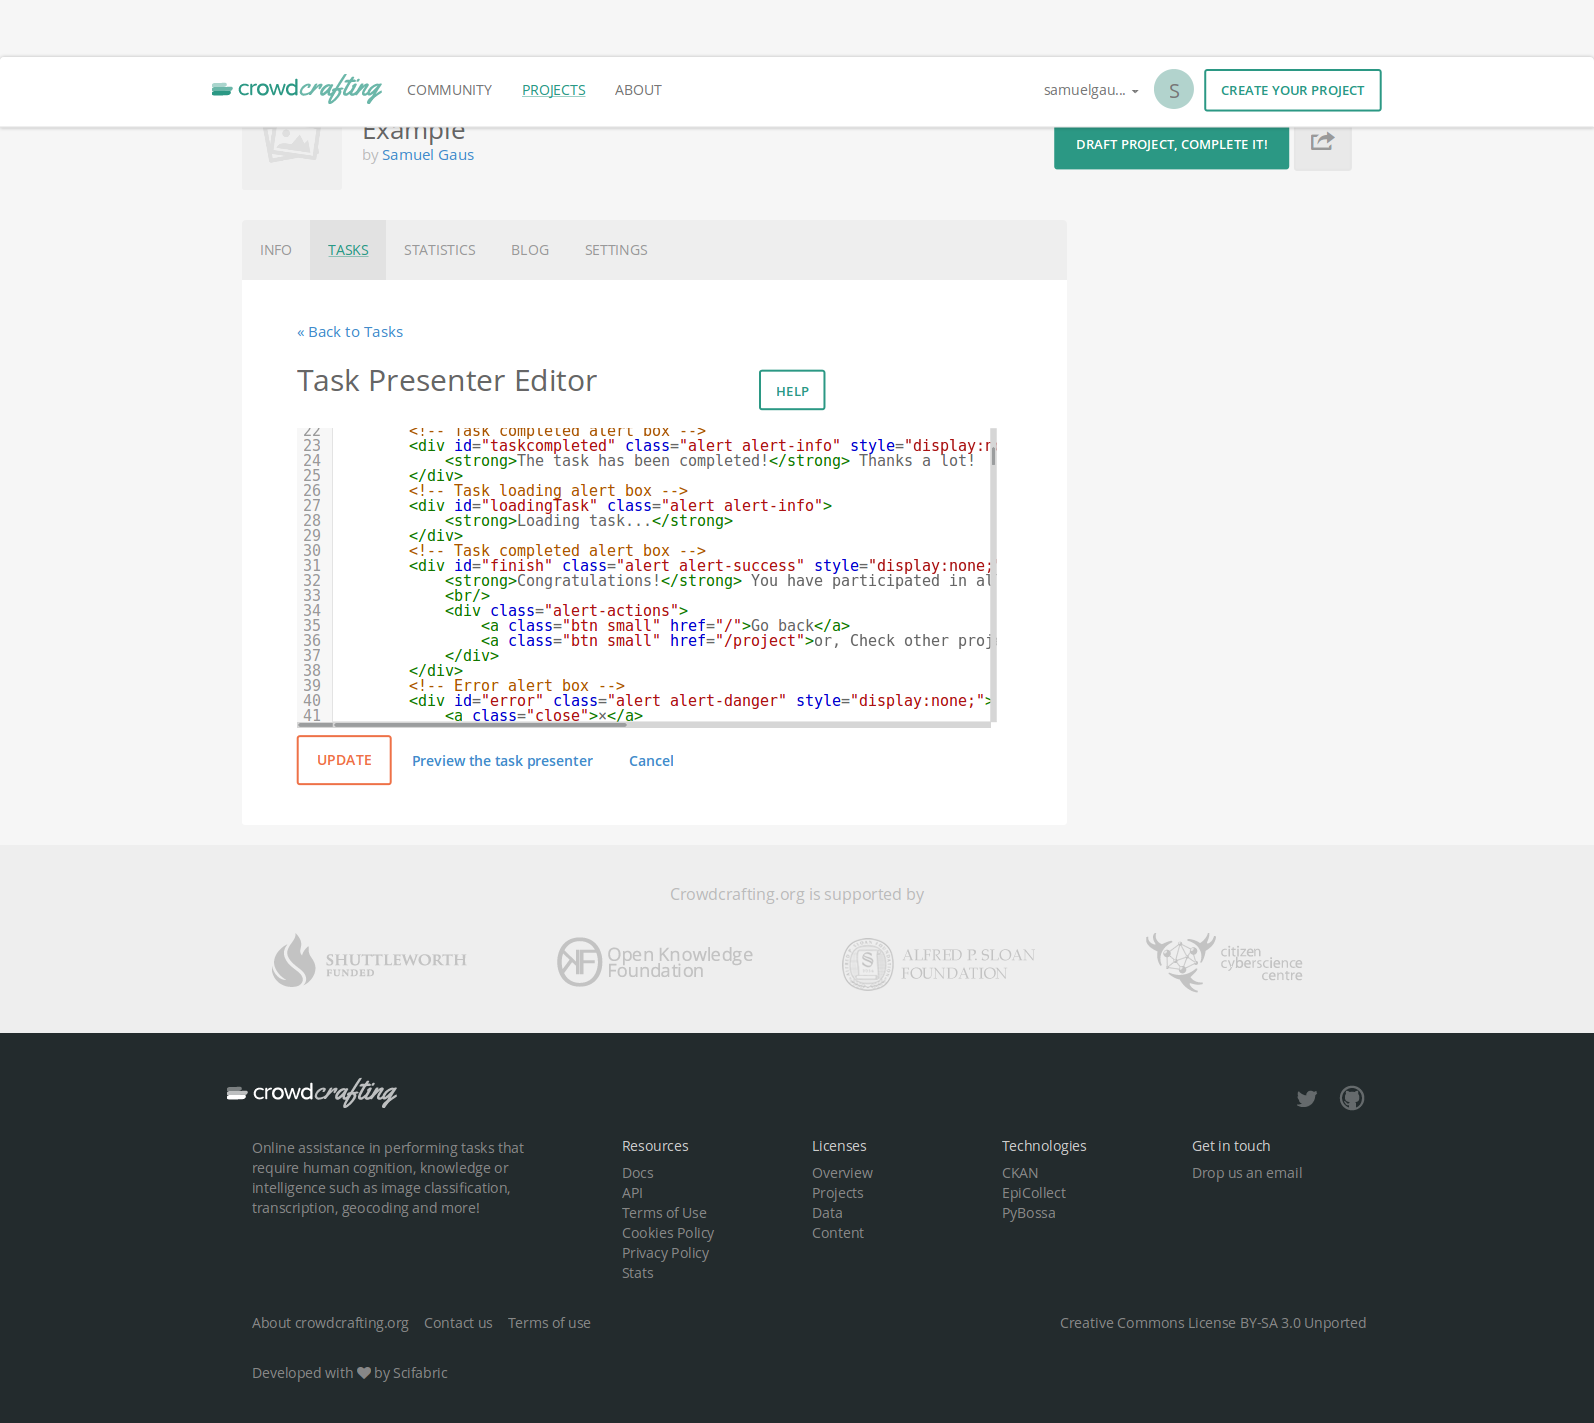
\includegraphics[width=4in]{cc-present}}
			\caption{Form creation screen in \emph{crowdcrafting}}
			\label{fig:cc-present}
		\end{figure}

		This would then create an input form for the data you wish to collect. However, because \emph{PyBOSSA} focusses on atomised tasks rather than a more general goal, it is not possible to create a question that any user can answer repeatedly. For example if you wanted to collect information about potholes, the task ``Where do you see a pothole?'' could be created. Once a user has `completed' this `task', however, they would not be able to answer it again, this causing the campaign to almost be one-use. Similarly, in the `Task Redundancy' settings area, you can specify how many times a single task can be repeated before closing. In the campaigns \emph{PyBOSSA} is built for, this would be to allow verification of submissions by seeing that multiple users provided the same data. In our example, however, it would be necessary to provide an arbitrary high number to allow the data collection to continue indefinitely.

		\subsubsection{FixMyStreet}

		\emph{FixMyStreet} is a much closer fit to the requirements in this study because it allows users to submit data on any location at a rate that they choose. Fortunately, the project is free\cite{_mysociety/fixmystreet_2015} and open source. However, the software itself is built specifically for reporting problems to a local authority and the back-end framework is very closely coupled with this concept and front-end. As a result, it would need heavy modification to work with a more generalised usage. This scale of modification required could be sufficient to justify building a new framework from the ground up, taking inspiration from \emph{FixMyStreet} rather than a straight fork of the codebase.

		\subsection{Conclusion}

		As was made clear when extracting the \hyperref[sec:common-functionalities]{common functionalities}, there is a huge overlap in the functionality of many crowdsourcing projects. There is a clear `type' of project for which a framework could be built that would save future campaign-creators having to make their own. This type of project - open submission of data with a geographic coordinate - is not well catered for by \emph{PyBOSSA}, which is built around finding a large task, atomising it into smaller tasks, and sharing them equally across the crowd. Even building something similar using \emph{PyBOSSA} would require significant technical knowledge to edit the HTML and JavaScript for the end-user to quickly enter data.

		A framework implementing the common functionalities could act as a level of abstraction away from these technical issues. From the analysis of the existing applications, a number of benefits can be drawn:

		\begin{enumerate}
			\pitem{Opening crowdsourcing to a wider audience} Currently there is some level of technical expertise required in setting up a crowdsourcing project of the type described. One either needs to be able to adapt existing open source technologies or write your own. Although this may be possible for some, it restricts the creation of crowdsourcing scenarios to those who have time and skill to dedicate to it.

			Crowdsourcing is meant to have the possibility of being casual - no one individual needs to carry the whole project because the data collection is shared by so many people. If this principal were applied to the creation of the campaign as well as the taking part, it's possible that much more data could be collected in general. Although this is not useful on its own clearly, if the collected data is open and available to the public it could be accessed easily by researchers. This is not without issue, however, as the casual nature of crowdsourcing has also been criticized academically\cite{brabham_myth_2012}.
			\pitem{Responding to time-critical data collection requirements} Even if one has the skill to apply to creating a crowdsourcing application to collect data, the campaign itself may be time critical. In a humanitarian crisis where data needs to be collected extremely quickly to be useful at all, it is much more preferable to have a system ready to be adapted to the specific needs and rolled out. For example, the usefulness of \emph{Tomnod} during the search for Malaysian Airlines Flight 370 would have been very little if it had come out several days later.
			\pitem{Saving money} A framework could save money for two reasons.
			\begin{itemize}
				\item Running and hosting pre-existing solutions costs money whereas a framework could offer a centralised platform (analogous to the relationship between \emph{PyBOSSA} and \emph{crowdcrafting}).
				\item These other problems can always be (and inevitably are) solved by spending money, either through hiring staff or learning new skills.
			\end{itemize}
			\pitem{Cross-pollination} If a centralised platform were hosted using this crowdsourcing platform, and they shared a web interface and mobile application, smaller campaigns would benefit for a number of reasons.
			\begin{itemize}
				\item Multiple campaigns could be accessed through the same interface. This means when a user is supplying information for a specific campaign of personal or public interest could be e
			\end{itemize}
		\end{enumerate}

	\section{Architecture}
	\label{sec:architecture}
		As a result of the analysis and background above, a framework could be produced to provide sufficient functionality to replace the bespoke implementations so far. The framework would need to consist primarily of an API that can receive submitted data, perform all the necessary back-end organisation of that data, and expose a way of interacting with inbuilt data. On top of that, it will be necessary to construct a number of front-ends to interact with the API - a web-based and a mobile application.

		\subsection{Requirements Analysis}

		This section contains a detailed and quantifiable list of the requirements for the framework, built from the common functionalities of the analysed projects.

		\newcounter{requirementcounter}
		\newcommand\rqrn{\stepcounter{requirementcounter}\arabic{requirementcounter}}

		\subsubsection{Users}

		\begin{tabular}{ | l | l | l | }
			\hline
			\textbf{\textnumero} & \textbf{Category} & \textbf{Requirement} \\ \hline
			& & Users must be able to...\\
			\rqrn & Authentication & Sign up.\\
			\rqrn & Authentication & Sign in.\\
			\rqrn & Authentication & Sign out.\\
			\rqrn & Authentication & Sign up and in using accounts from social media.\\
			\rqrn & Authentication & Reset their passwords.\\
			\rqrn & Authentication & Delete their accounts.\\
			\rqrn & Profiles & Edit their user profiles.\\
			\rqrn & Profiles & Find other users.\\
			\rqrn & Campaigns & Join a campaign.\\
			\rqrn & Campaigns & Leave a campaign.\\
			\hline
		\end{tabular}

		\begin{itemize}
			\item What the project is
			\item Requirements analysis - very fine detail. Almost like an API per requirement. Basically walk through actions and almost describe each API call that would need to happen (kind of).
			\item Component diagram. Do not specify technologies (this is for later).
			\item How it works.
			\item Technologies used and why.
			\item Describe Full API docs in appendices.
		\end{itemize}

	\section{Implementation}
	\label{sec:implementation}
		\begin{itemize}
			\item Link to repository.
			\item Link to a working implementation. http://croud.io/.
			\item JSON schema.
			\item Key snippets of code for each component - for each component show a front-end screen and maybe some code that powers it.
			\item Special features that might take effort from new developers.
			\begin{itemize}
				\item Offline caching
				\item Moderation
				\item Stale.
			\end{itemize}
		\end{itemize}

	\section{Evaluation}
	\label{sec:evaluation}
		\begin{itemize}
			\item Show it using two completely different campaigns.
			\item Explain why you chose the two campaigns you did and list their requirements.
			\item Walkthrough of how user would create a campaign (with screenshots and links ideally)
			\item Walkthrough of how data is submitted
		\end{itemize}
	\section{Conclusion}
	\label{sec:conclusion}
		\begin{itemize}
			\item Future changes that could be added.
			\item Conclude that it works etc etc
		\end{itemize}

	\bibliographystyle{Croud}
	\bibliography{Croud}

\end{document}
